\subsection{model}
\label{subsec:model}

\begin{figure}[H]
  \centering
  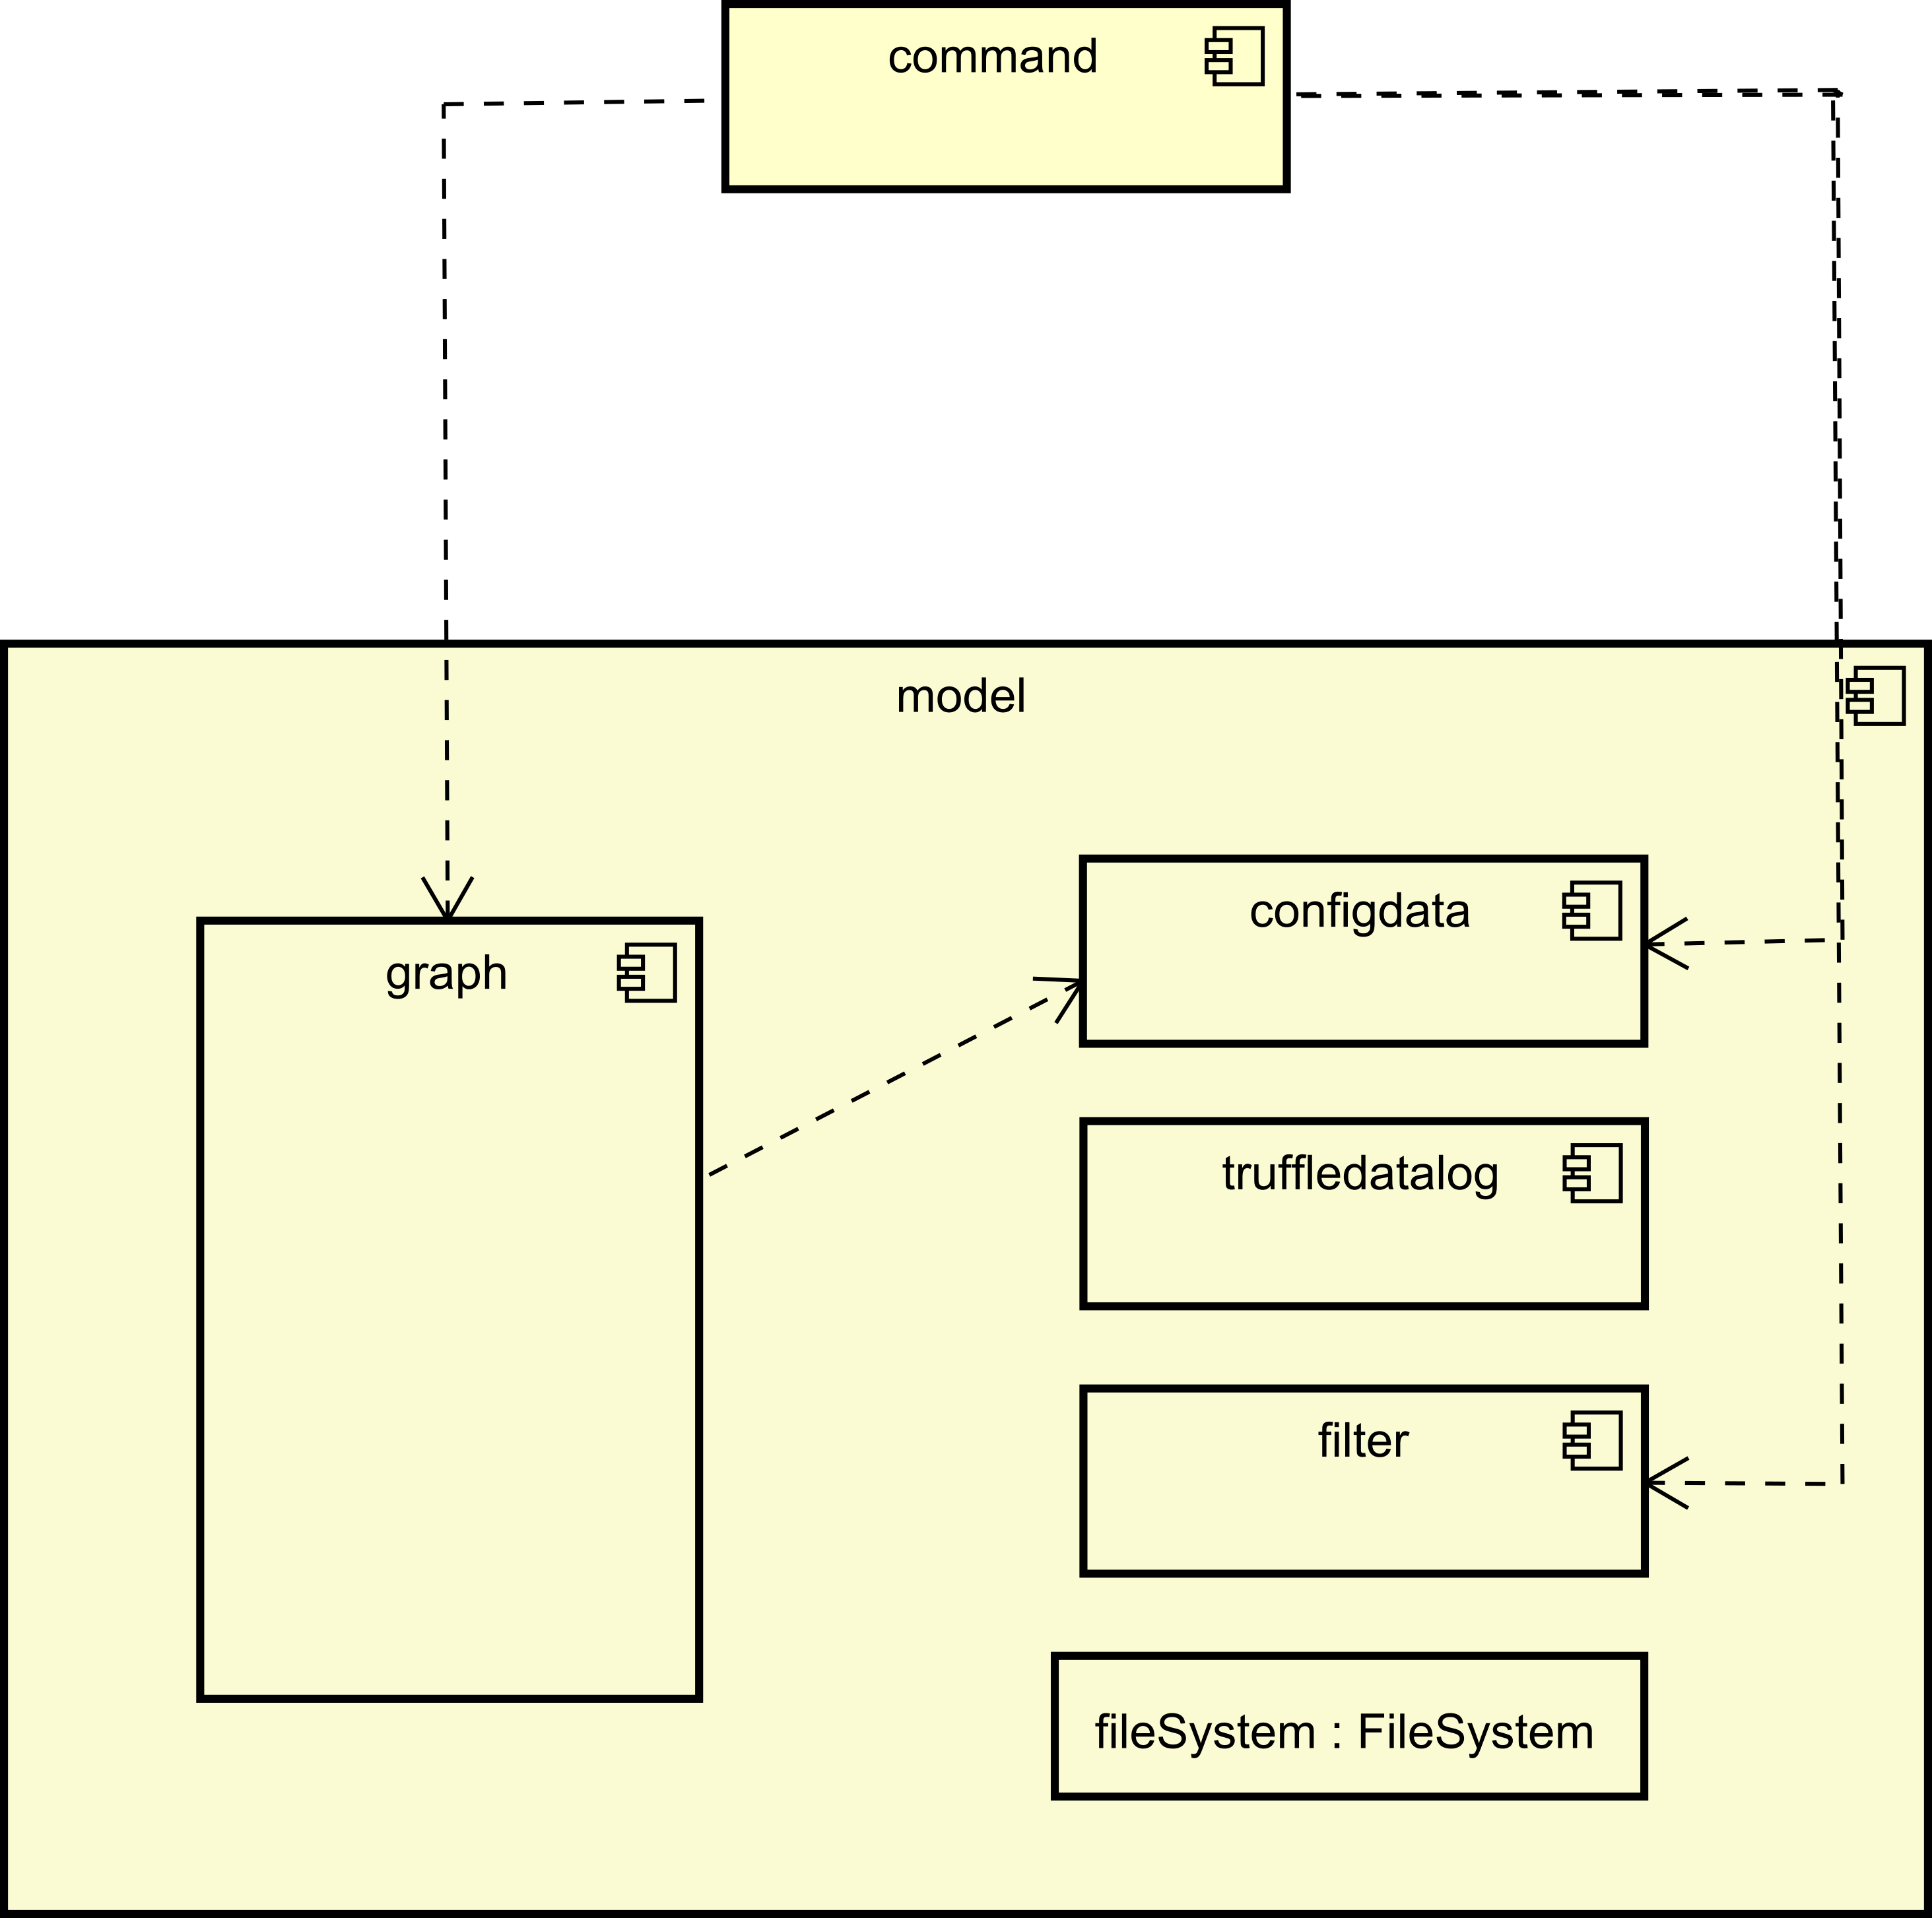
\includegraphics[width=\textwidth]{../diagramimages/model.png}
  \caption{model-Package}
\end{figure}

\medskip
Das Model beinhaltet jegliche Datenstrukturen, die von \gls{programname} genutzt
werden. Zum Beispiel ist sowohl der Graph, welcher im View angezeigt wird,
als auch alle Konfigurationen, die der Benutzer eingestellt hat, hier enthalten. Wir haben uns
dafür entschieden dem Model keine Ausführungslogik zu geben.
D.h. es besitzt kein eigenen Thread und wird wie eine Datenstruktur von den
\hyperref[subsec:service]{Services} und dem \hyperref[subsec:view]{View} verwendet.

    \subsubsection{graph}
    \label{subsubsec:graph}

    Dieses Unterpackage macht das eigentliche Modell aus. Der gesamte Graph sowie
    all seine möglichen Layouts, entsprechende Interfaces und ein Proxy aus dem
    \gls{proxypattern} für die Entkopplung sind hier enthalten.\par
    Wir haben uns dazu entschieden, ein Graphobjekt immer als Proxy zu übergeben, da es damit einfach wird,
    bei sämtlichen Benutzern des Objekts, die Referenz auf den Graph umzubiegen. Dies ist zum Beispiel
    für die Replayfunktion nützlich. Wenn ein bestimmter Zustand geladen wird, so wird ein serialisiertes
    Graphobjekt von der Festplatte geladen und deserialisiert. Anschliesend wird der Graphproxy
    umgestellt, sodass er auf das neue Graphobjekt zeigt. Damit ist zum Beispiel keine Änderung direkt in der View vonnöten.\par
    Der NetworkGraphSwitch ist im Prinzip auch eine Art Proxy. Der Unterschied liegt hierbei darin, dass
    er immer zwei Referenzen auf zwei GraphProxies hält. Dies ist insofern sinnvoll, dass es dann einfach wird
    den Graphen umzustellen, den die View darstellen soll: Im Programm sind durch die Replayfunktion zwei
    Graphinstanzen vorhanden. Die eine ist für die aktuell ankommenden Daten zuständig, und die andere realisiert
    die Replayfunktion. Falls nun der Nutzer auf Playback wechselt, so muss lediglich bei dem NetworkGraphSwitch
    viewPlayback aufgerufen werden.

    \clearpage
    \begin{sidewaysfigure}
      \centering
      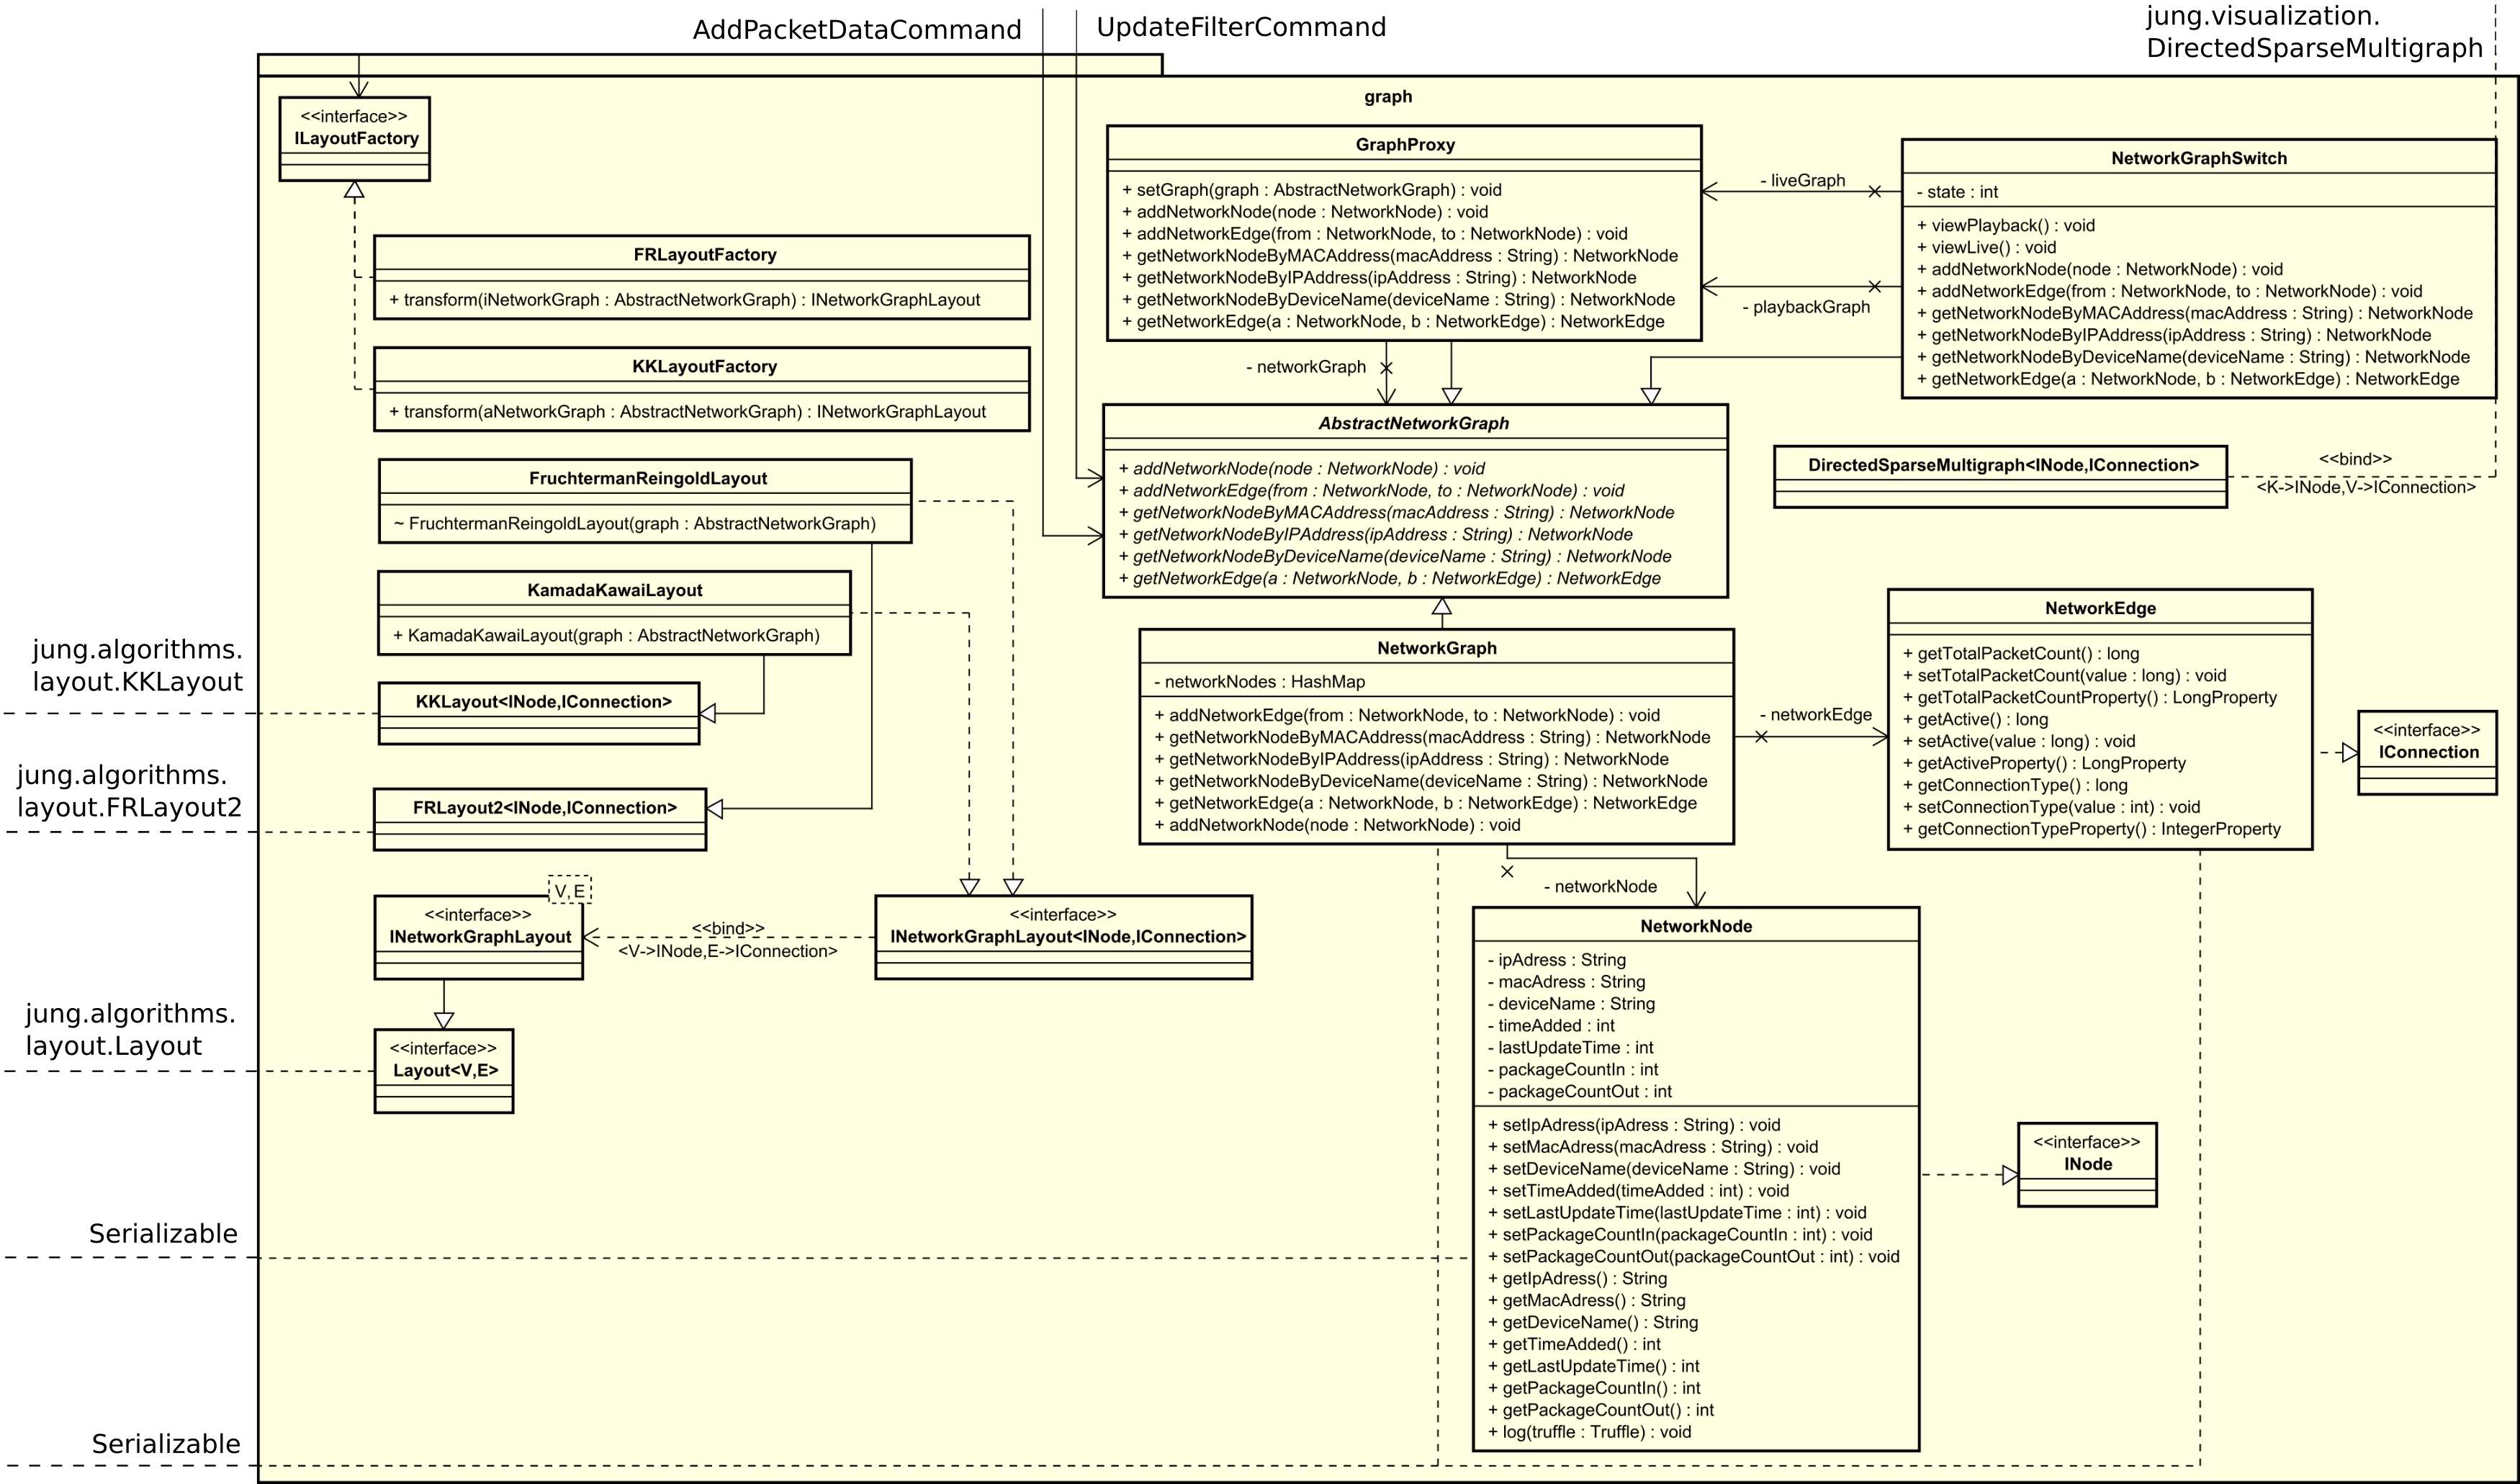
\includegraphics[width=\textwidth]{../diagramimages/graph.png}
      \caption{graph-Package}
    \end{sidewaysfigure}
    \clearpage

    \subsubsection{filter}
    \label{subsubsec:filter}

    \begin{figure}[H]
      \centering
      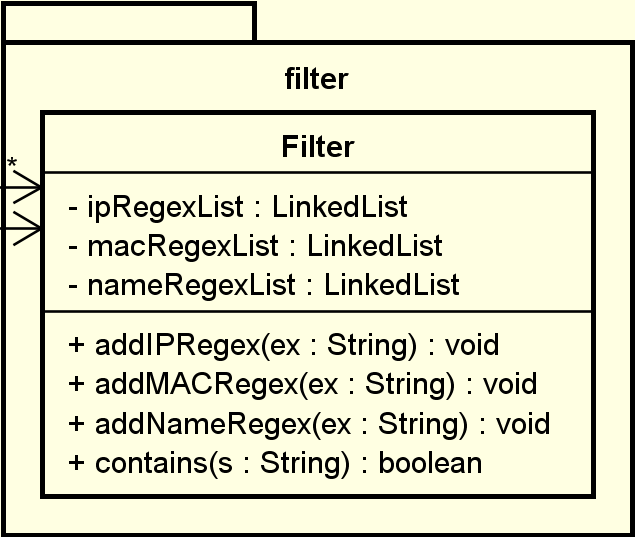
\includegraphics[width=0.5\textwidth]{../diagramimages/filter.png}
      \caption{filter-Package}
    \end{figure}

    \medskip
    Das filter-Package beinhaltet eine \textit{Filter}-Klasse, die in der Lage ist,
    Knoten basierend auf vom Nutzer gesetzen Kriterien zu klassifizieren. Verschiedene
    Klassifikationen werden verschieden in der \gls{gui} dargestellt. So kann
    Beispielsweise eine Blacklist oder Whitelist erstellt werden.
    Natürlich kann der Benutzer basierend auf \gls{ip}- und \gls{mac}-Addressräumen,
    Gerätenamen oder Knotenselektionen seine eigenen Filter definieren.

    \subsubsection{configdata}
    \label{subsubsec:configdata}

    \begin{figure}[H]
      \centering
      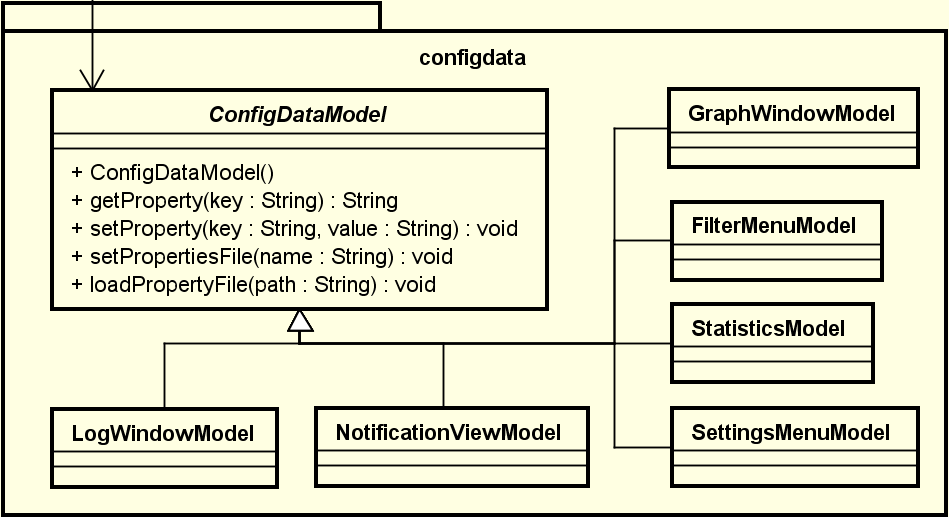
\includegraphics[width=\textwidth]{../diagramimages/configdata.png}
      \caption{configdata-Package}
    \end{figure}

    \medskip
    Im configdata-Package werden jegliche Konfigurationen gespeichert, hin von den
    Beschriftungen der Bedienelemente in der \gls{gui} bis zu den erstellten Filterlisten. Dieses
    wird zum Großteil durch Java Property Files gemacht, welche den Vorteil haben, dass
    sie mit Java Propertyobjekten gekoppelt sind und dadurch leicht auszutauschen sind.
    Das heißt, wenn der Benutzter beispielsweise die Sprache des Programms ändern
    will, so muss intern nur eine andere Property File geladen werden.
    \newline
    \newline
    Der Aufbau dieses Packages setzt sich aus einer abstrakten Oberklasse
    \textit{ConfigDataModel} zusammen, die das Zusammenspiel zwischen Property Files
    und Propertyobjekten verwaltet. Jedes \gls{gui}-Element, welches Daten anzeigt, hat
    ein JavaFX Property-Binding mit einer Unterklasse, die \textit{ConfigDataModel}
    bererbt. So wird automatisch die \hyperref[subsec:view]{View} aktualisiert,
    wenn sich das darunterliegende ConfigDataModel-Objekt ändert. D.h.
    \textit{FilterMenuModel} beinhaltet alle Konfigurationsdaten inklusiver der
    Filterlisten des Filtermenüs. Das Gleiche gilt für alle anderen Menüs und
    deren Models.


    \subsubsection{truffledatalog}
    \label{subsubsec:graphlog}

    \begin{figure}[H]
      \centering
      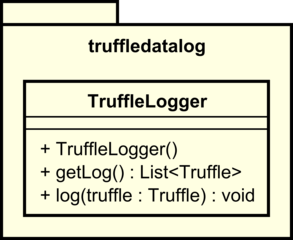
\includegraphics[width=0.5\textwidth]{../diagramimages/truffledatalog.png}
      \caption{turffledatalog-Package}
    \end{figure}

    \medskip
    Das truffledatalog-Package beinhaltet eine \textit{TruffleLogger}-Klasse, von
    welcher jeder Knoten eine Instanz besitzt. Diese wird beim Eintreffenden neuer Truffles
    (oder Commands) benutzt um die neuen Daten des Truffles in einer Text- oder xml-Datei zu speichern,
    sodass bei Bedarf genau gesehen werden kann, was für \glspl{paket} bei einem
    Knoten eingetroffen sind. D.h., dass jeder Knoten seine eigene Text- oder xml-Datei
    hat, wo genau drin steht was für \glspl{paket} dieser schon erhalten hat,
    von wem, etc.